% --------------------------------------------------------------
%     DENNE MALEN ER LAGET AV MARTIN SORIA RØVANG
%     TIL BRUK FOR OPPGAVELØSNINGER OG RAPPPRTER
%     GITHUB: github.com/martinrovang
% --------------------------------------------------------------


\documentclass[12pt]{article}
\usepackage{amsmath,amsthm,amssymb}
\usepackage{float}
\usepackage[norsk]{babel}
\usepackage[table]{xcolor}
\usepackage{color}
\usepackage{graphicx}
\usepackage{listings}
\usepackage{natbib}
\usepackage[utf8]{inputenc}
\usepackage{imakeidx}
\usepackage[a4paper]{geometry}
\usepackage[myheadings]{fullpage}
\usepackage{fancyhdr}
\usepackage{lastpage}
\usepackage{graphicx, wrapfig, subcaption, setspace, booktabs}
\usepackage[T1]{fontenc}
\usepackage[font=small, labelfont=bf]{caption}
\usepackage{fourier}
\usepackage[protrusion=true, expansion=true]{microtype}
\usepackage{url, lipsum}
\usepackage{tgbonum}
\usepackage{hyperref}
\usepackage{xcolor}
\usepackage[most]{tcolorbox}
\usepackage{mathtools}
\usepackage[page]{totalcount}
\usepackage{lastpage}
\usepackage{pgfplots}


\newcommand{\HRule}[1]{\rule{\linewidth}{#1}}
\onehalfspacing
\setcounter{tocdepth}{5}
\setcounter{secnumdepth}{5}
\newcommand{\vect}[1]{\boldsymbol{#1}}

\definecolor{codegreen}{rgb}{0,0.6,0}
\definecolor{codegray}{rgb}{0.5,0.5,0.5}
\definecolor{codepurple}{rgb}{0.58,0,0.82}
\definecolor{backcolour}{rgb}{0.95,0.95,0.92}
\definecolor{skyblue}{rgb}{0.950, 1, 1}

\lstdefinestyle{mystyle}{
    backgroundcolor=\color{backcolour},   
    commentstyle=\color{codegreen},
    keywordstyle=\color{magenta},
    numberstyle=\tiny\color{codegray},
    stringstyle=\color{codepurple},
    basicstyle=\footnotesize,
    breakatwhitespace=false,         
    breaklines=true,                 
    captionpos=b,                    
    keepspaces=true,                 
    numbers=left,                    
    numbersep=5pt,                  
    showspaces=false,                
    showstringspaces=false,
    showtabs=false,                  
    tabsize=2,
    frame=single,
    %keywordstyle=\color{blue},
    language=Python,
    backgroundcolor = \color{skyblue}
}
 
\lstset{style=mystyle}
\lstset{
    basicstyle=\footnotesize\ttfamily,
  identifierstyle=\bfseries\color{green!40!black},
  commentstyle=\itshape\color{purple!40!black},
  keywordstyle=\color{blue},
  stringstyle=\color{orange},
}

\newcommand{\N}{\mathbb{N}}
\newcommand{\Z}{\mathbb{Z}}
 
\newenvironment{theorem}[2][Theorem]{\begin{trivlist}
\item[\hskip \labelsep {\bfseries #1}\hskip \labelsep {\bfseries #2.}]}{\end{trivlist}}
\newenvironment{lemma}[2][Lemma]{\begin{trivlist}
\item[\hskip \labelsep {\bfseries #1}\hskip \labelsep {\bfseries #2.}]}{\end{trivlist}}
\newenvironment{exercise}[2][Exercise]{\begin{trivlist}
\item[\hskip \labelsep {\bfseries #1}\hskip \labelsep {\bfseries #2.}]}{\end{trivlist}}
\newenvironment{problem}[2][Problem]{\begin{trivlist}
\item[\hskip \labelsep {\bfseries #1}\hskip \labelsep {\bfseries #2.}]}{\end{trivlist}}
\newenvironment{question}[2][Question]{\begin{trivlist}
\item[\hskip \labelsep {\bfseries #1}\hskip \labelsep {\bfseries #2.}]}{\end{trivlist}}
\newenvironment{corollary}[2][Corollary]{\begin{trivlist}
\item[\hskip \labelsep {\bfseries #1}\hskip \labelsep {\bfseries #2.}]}{\end{trivlist}}

\newenvironment{solution}{\begin{proof}[Solution]}{\end{proof}}
    
\makeindex[columns=3, title=Alphabetical Index, intoc]


% --------------------------------------------------------------
%                         Headers and footers
% --------------------------------------------------------------
\fancyhf{}
\pagestyle{fancy}
\rhead{Martin Soria Røvang}
\lhead{STA-2003-Tidsrekker}
\rfoot{Side \thepage \, av \pageref{LastPage}}
\renewcommand{\headrulewidth}{0.3pt}

\begin{document}
% --------------------------------------------------------------
%                         FRONTPAGE
% --------------------------------------------------------------
{\fontfamily{cmr}\selectfont
\title{ \normalsize \textsc{}
		\\ [3.0cm] % How much upper margin
		%\HRule{0.5pt} \\
        \LARGE \textbf{\uppercase{Obligatorisk Oppgave 1}
        \HRule{0.5pt} \\ [0.5cm]
        STA-2003-Tidsrekker
        %\HRule{2pt} \\ [0.5cm]
        \\
		\normalsize \today \vspace*{5\baselineskip}}
		}

        \date{}
\author{
		Martin Soria Røvang \\ 
        Universitetet i Tromsø \\}

% \begin{titlepage}
\clearpage\maketitle
\vspace{0.2\textheight}
{\centering
Inneholder \pageref{LastPage} \, sider, inkludert forside.\par
}
\thispagestyle{empty}
% \end{titlepage}

\newpage
\tableofcontents
% --------------------------------------------------------------
%                         Start here
% --------------------------------------------------------------


\newpage

\section{Oppgave}
\subsection{a}

Replace this text with your summary/reflection of ``The Secret to Raising Smart Kids".  Your total reflection should be roughly a page long.
 
Kodetest:\newline

\begin{figure}[hbt!]
\begin{lstlisting}
def fps_check(self, time1, frames, lastframe):
    """Finds the FPS, returns time, current frame and last FPS frame"""
    time2 = time.clock()
    # If one second has passed return new FPS.
    if (time2 - time1) > 1:
        lastframe = frames
        frames = 0
        time1 = time.clock()
        return time1, frames, lastframe
    else:
        frames += 1
        return time1, frames, lastframe
\end{lstlisting}
\caption{Kode caption}
\label{Kode1}
\end{figure}

Referanse til kode \ref{Kode1}



\begin{equation}
    \int_{0}^{x} x^{2} \, dx
\end{equation}


\begin{equation}
    \Omega = 505
\end{equation}


\begin{figure}[hbt!]
    \centering
    
\includegraphics{test.png}
    \caption{testbilde}
    \label{test_image}
\end{figure}

Dette er en referanse til testbildet \ref{test_image}.


\newpage
Vektortester:
\begin{equation}
    \vect{B} = (1000,500)
\end{equation}
\begin{equation}
    \vec{B} = (1000,500)
\end{equation}

Ligning uten referanse

\begin{equation*}
    \nabla F = 5
\end{equation*}

Dette er en referanse test [p.38 \cite{alpaydin_2014}]


Dette er en link \url{www.google.no}\footnote{Dette er en linktest i footer \url{www.google.no}}

\newpage

\section{Oppgave}
\subsection{a}

Ny seksjonstest.


\begin{figure}[hbt!]
    \centering
    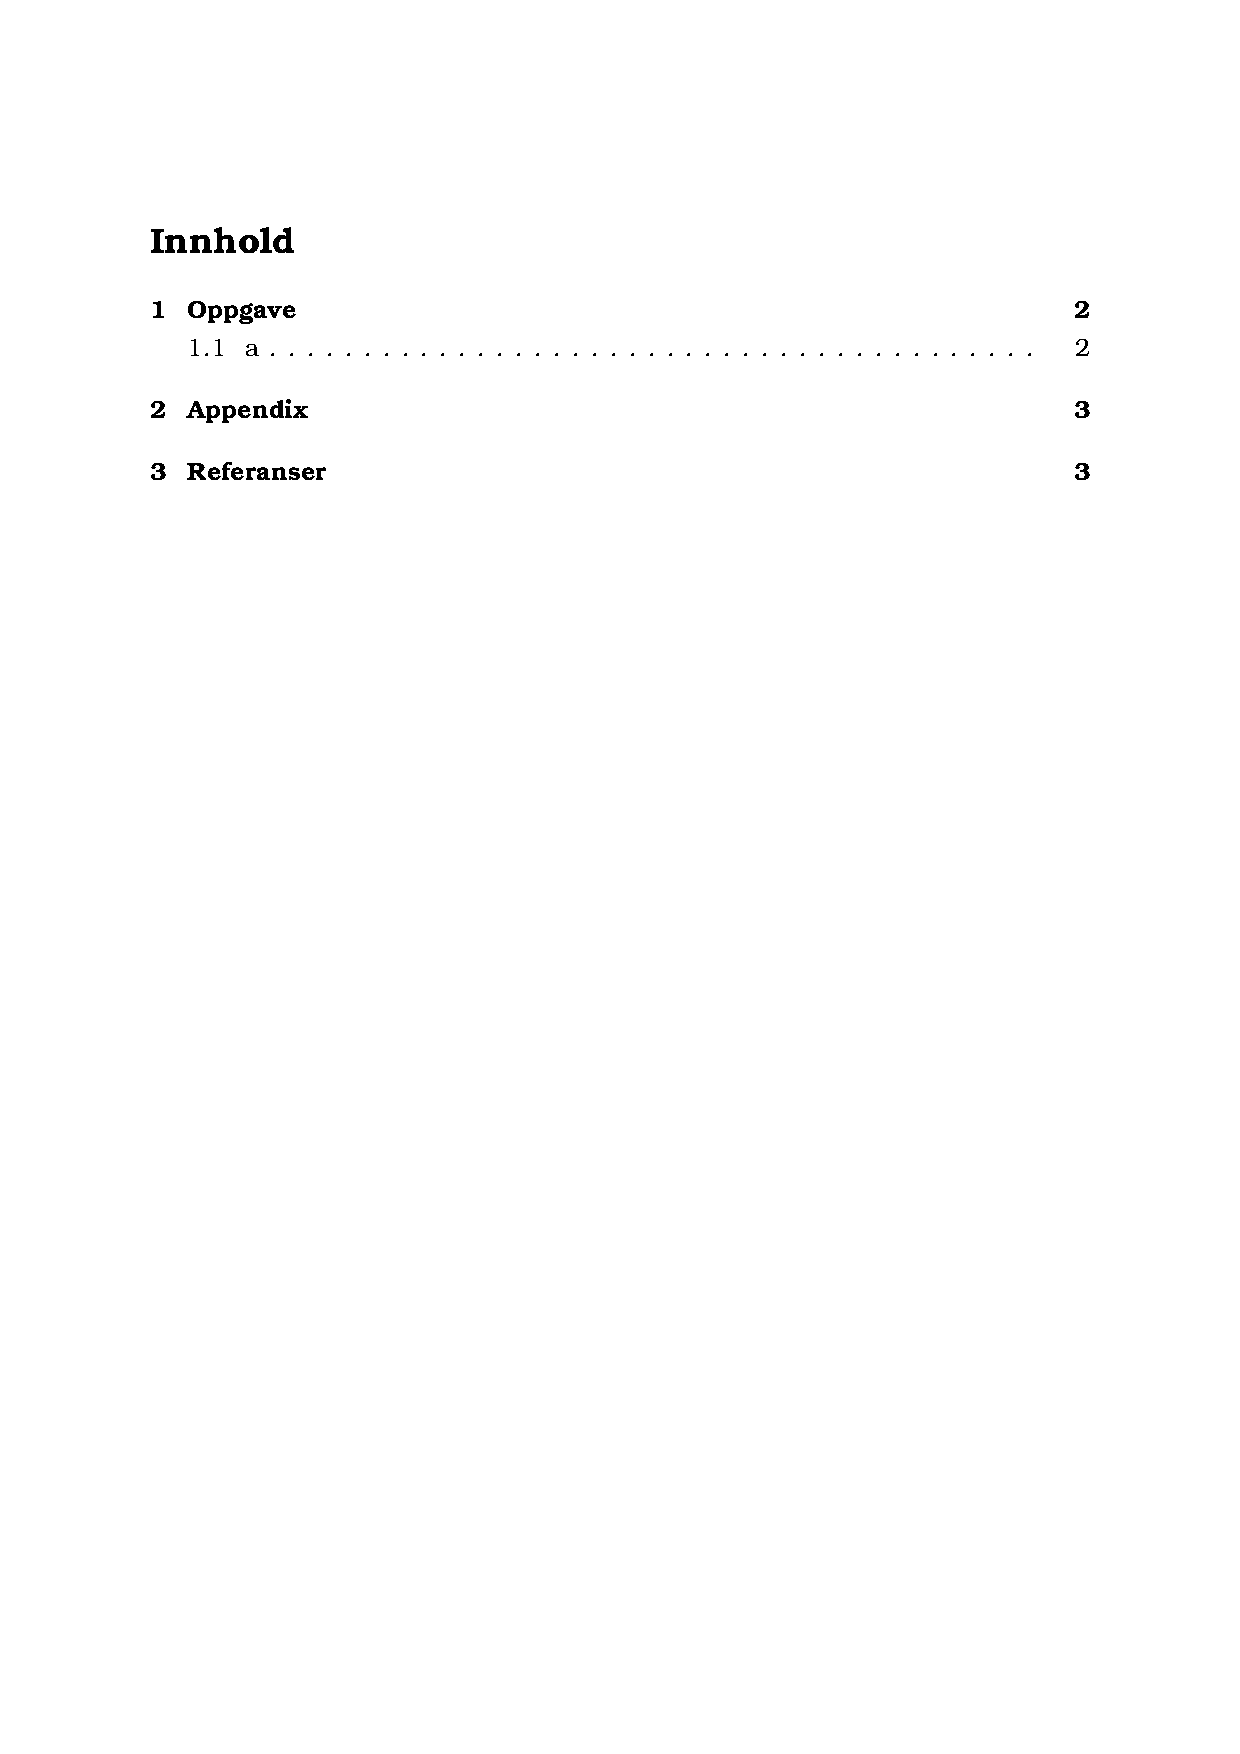
\includegraphics{test.pdf}%[width=0.5\textwidth]
    \caption{testbilde}
    \label{test_image}
\end{figure}


% --------------------------------------------------------------
%     Reference og appendix
% --------------------------------------------------------------
\newpage
\section{Appendix}
\section{Referanser}
\begingroup
\renewcommand{\section}[2]{}%
%\renewcommand{\chapter}[2]{}% for other classes
\bibliographystyle{plainnat}
\bibliography{bibl}
\endgroup




% --------------------------------------------------------------
%     You don't have to mess with anything below this line.
% --------------------------------------------------------------
 





\end{document}

